
\section{Supplementary Material}
Included here are the supplementary figures and tables for Chapter 2.
\linespread{1}
\begin{sidewaystable}
\caption[Summary of recombination rates per chromosomes]{Summary of sex-averaged recombination rates \emph{M. m castaneus} compared with the rates from Brunschwig et al. (2012) and Cox et al. (2009). Rates for the castaneus and Brunschwig maps are presented in terms of $4N_{e}r/bp$. Estimates of $N_e$ were obtained by assuming the recombination rates from Cox et al. (2009).}
 \begin{tabular}{c c c c c c c c c } 
  \hline
& & &  & & \multicolumn{3}{c}{Switch Errors} &  \\
Filter Set & HWE & Min DP & Max DP & Min GQ & H40 & H46 & H62 & \\ \hline
1 & - & - & - & - & 5,148/409,486 & 4,819/407,422 & 5,020/394,778 & 0.0124 \\
2 & <0.0002 & 10 & - & 15 & 1,690/338,592 & 1,451/334,111 & 1,452/324,199 & 0.0046 \\
3 & <0.0002 & 10 & 100 & 5 & 2,460 /341,744 & 2066 /339,508 & 2536 /328,998 & 0.0070 \\
4 & <0.0002 & - & - & 40 & 523 /288,471 & 444 /286,636 & 550 /281,266 & 0.0018 \\
 \hline
\end{tabular}    
 \label{tab:C2ST1}
\end{sidewaystable}

	
\begin{table}[h!]
\centering
\caption[Parameters of the best-fitting demographic model estimated from the analysis of 4-fold and CNE-flanking sites]{Parameters of the best-fitting demographic model estimated from the analysis of 4-fold and CNE-flanking sites. }
 \begin{tabular}{c c c c c } 

\toprule
	&4-fold	&CNE-flank \\ \hline
N2/N1&	0.40&	0.07 \\
t2/N1&	0.44&	0.17 \\
N3/N1&	0.40&	1.00 \\
t3/N1&	1.10&	0.63 \\
\bottomrule

\end{tabular}
\label{tab:CS2}
\end{table}
\begin{table}[h!]
\centering
\caption[Parameters of the 3-epoch demographic model at different sample sizes]{Parameters of the 3-epoch demographic model at different sample sizes. Down sampled datasets were generated by randomly selecting alleles, with respect to frequency, from the full dataset of 10 individuals.}
 \begin{tabular}{c c c c c } 

\toprule
\multirow{2}{*}{Parameter} & \multicolumn{3}{c}{Number of alleles sampled} \\ 
	&	$n = 10$ & 	$n = 16$ & 	$n = 20$ \\ \hline
N2/N1 &	0.030 &	0.030 &	0.060 \\
t2/N1 &	0.204 &	0.140 &	0.181 \\
N3/N1 &	0.120 &	0.200 &	0.800 \\
t3/N1 &	0.080 &	0.220 &	0.461 \\
\bottomrule

\end{tabular}
\label{tab:CS3}
\end{table}


\begin{table}
\caption{The overlap between the hotspots we identified in M. m. castaneus and the locations of DSB hotspots in wild-derived strains obtained by Smagulova et al. (2016). The corrected overlap is the number of overlapping hotspots, above the null expectation, over the total.}
\begin{tabular} {c c c c c c c} \\ [ 0.5ex ] \hline

\makecell{Strain\\ID} & Sub-species & \makecell{\# DSB \\ Hotspots} & \makecell{\# \\ Overlaps} & \makecell{\% Overlap \\ Uncorrected} & \makecell{Null \\Expectation} & \makecell{\% Overlap \\ Corrected}\\ \hline
13R & \emph{domesticus} & 14744 & 1202 & 8.2 & 1169 & 0.2 \\
B6 & \emph{domesticus}& 19455 & 1533 & 7.9 & 1505 & 0.1 \\ 
C3H & \emph{domesticus} & 14635 & 1399 & 9.6 & 1308 & 0.6 \\
CAST & \emph{castaneus} & 15061 & 1831 & 12.2 & 1221 & 4.1 \\
MOL & \emph{molossinus} & 15718 & 1559 & 9.9 & 1351 & 1.3 \\
PWD & \emph{musculus} & 14483 & 1569 & 10.8 & 1205 & 2.5 \\ \hline


\end{tabular}
\end{table}

 
 \begin{figure}
   \centering      
   \noindent\makebox[\textwidth]{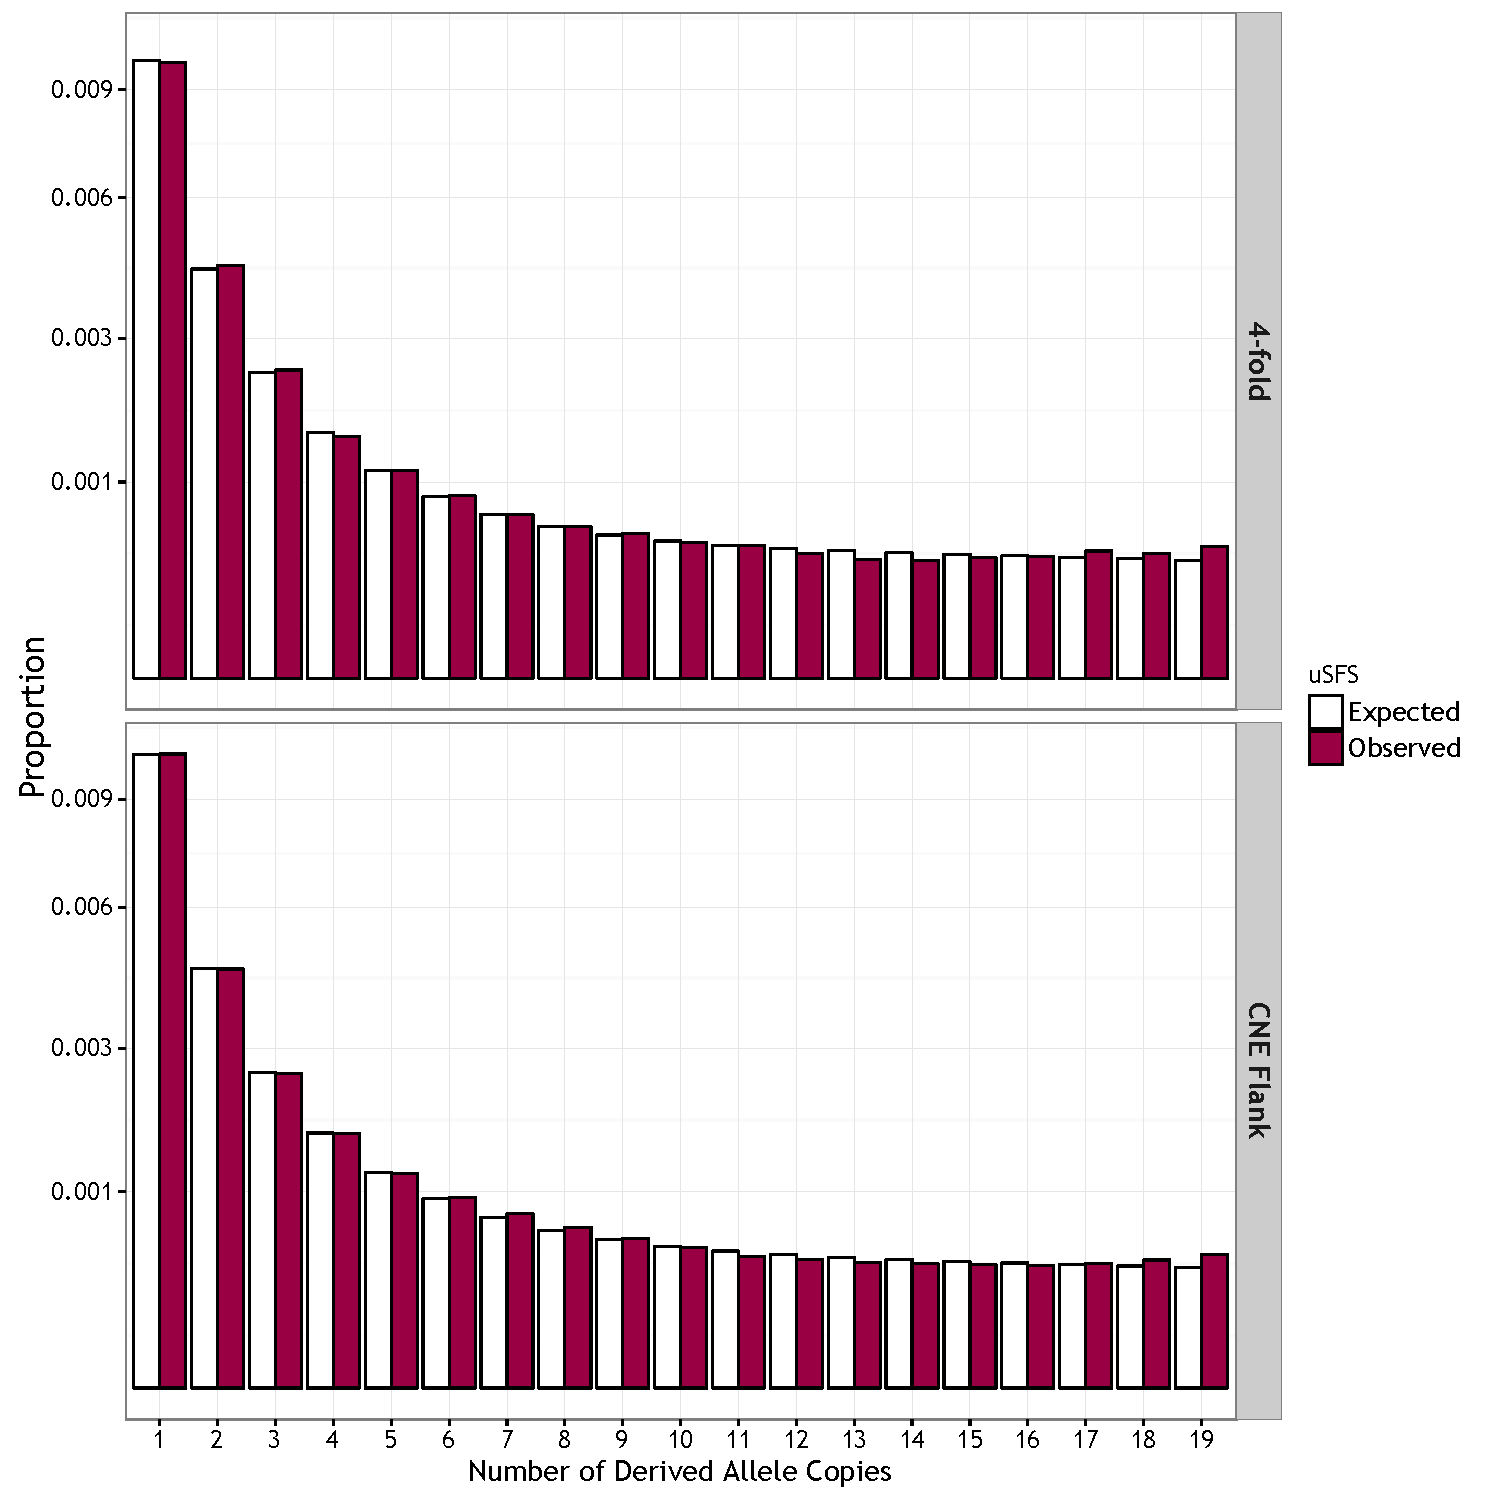
\includegraphics[width=\textwidth]{/Users/s0784966/Dropbox/Thesis/chapter2Appendix/Figures/FigureS1.pdf}}
 \caption[]{}
 \label{fig:1}
\end{figure}

 
 \begin{figure}
   \centering      
   \noindent\makebox[\textwidth]{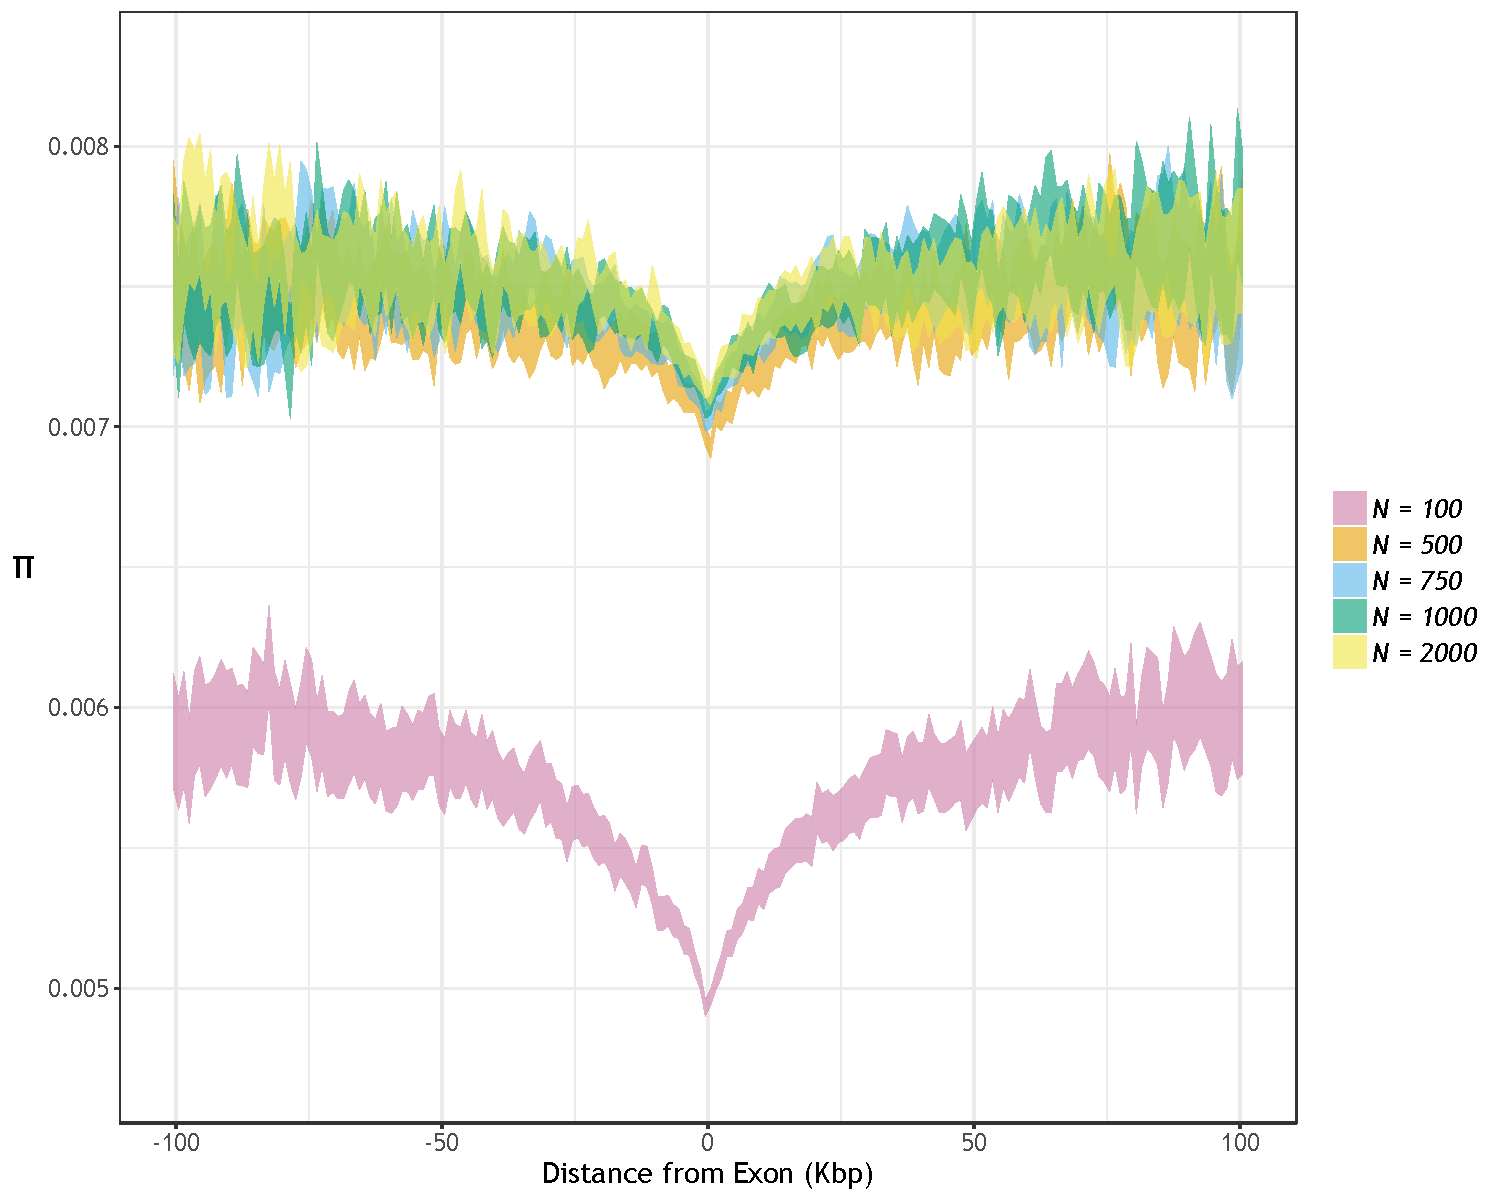
\includegraphics[width=\textwidth]{/Users/s0784966/Dropbox/Thesis/chapter2Appendix/Figures/FigureS2.pdf}}
 \caption[The effect of switch errors on recombination rate inference]{The effect of switch errors on the mean recombination rate inferred using LDhelmet with a block penalty of 100. Each black point represents results for a window of 4000 SNPs, with 200 SNPs overlapping between adjacent windows, using sequences simulated in SLiM for a constant value of $\rho/bp$. Red points are mean values. Switch errors were randomly incorporated at heterozygous SNPs with probability 0.0046. The dotted line shows the value when the inferred and true rates are equal}
 \label{fig:1}
\end{figure}

 
 \begin{figure}
   \centering      
   \noindent\makebox[\textwidth]{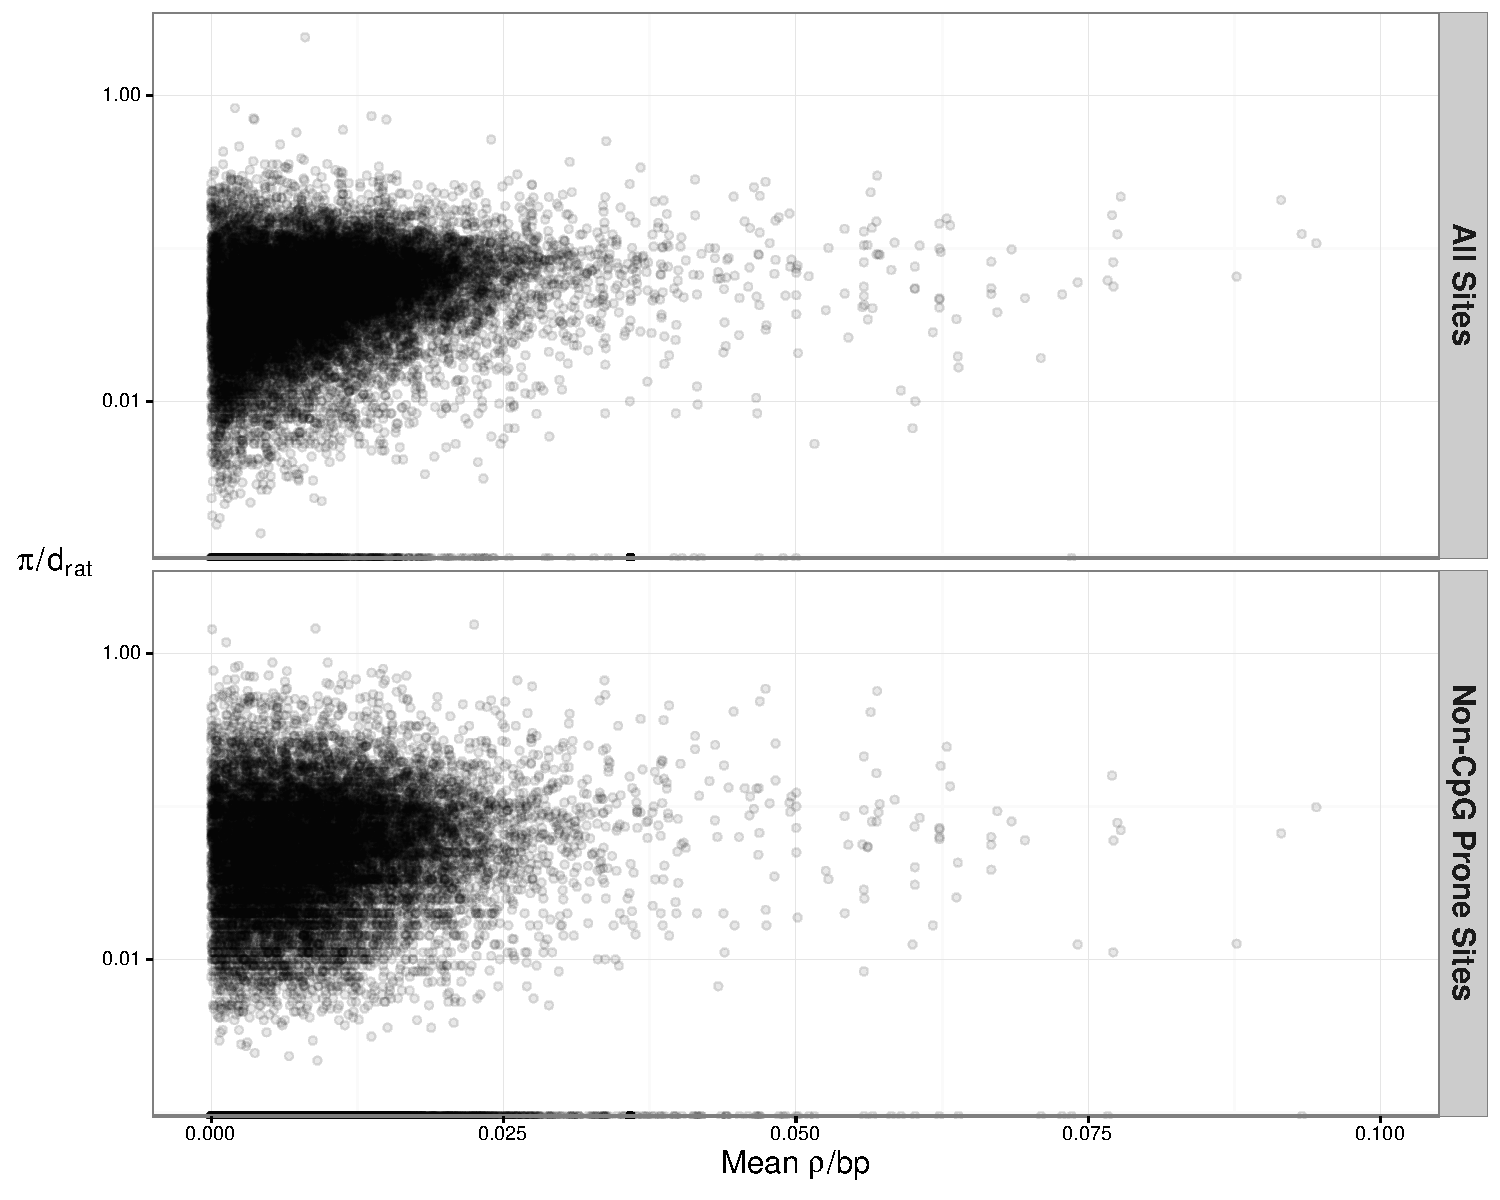
\includegraphics[width=\textwidth]{/Users/s0784966/Dropbox/Thesis/chapter2Appendix/Figures/FigureS3.pdf}}
 \caption[The effect of switch errors on recombination rate inference]{The effect of switch errors on the mean recombination rate inferred using LDhelmet with a block penalty of 100. Each black point represents results for a window of 4000 SNPs, with 200 SNPs overlapping between adjacent windows, using sequences simulated in SLiM for a constant value of $\rho/bp$. Red points are mean values. Switch errors were randomly incorporated at heterozygous SNPs with probability 0.0046. The dotted line shows the value when the inferred and true rates are equal}
 \label{fig:1}
\end{figure}

\linespread{2}
\pagebreak
\section{Booker \emph{et al.} 2017 - Genetics}
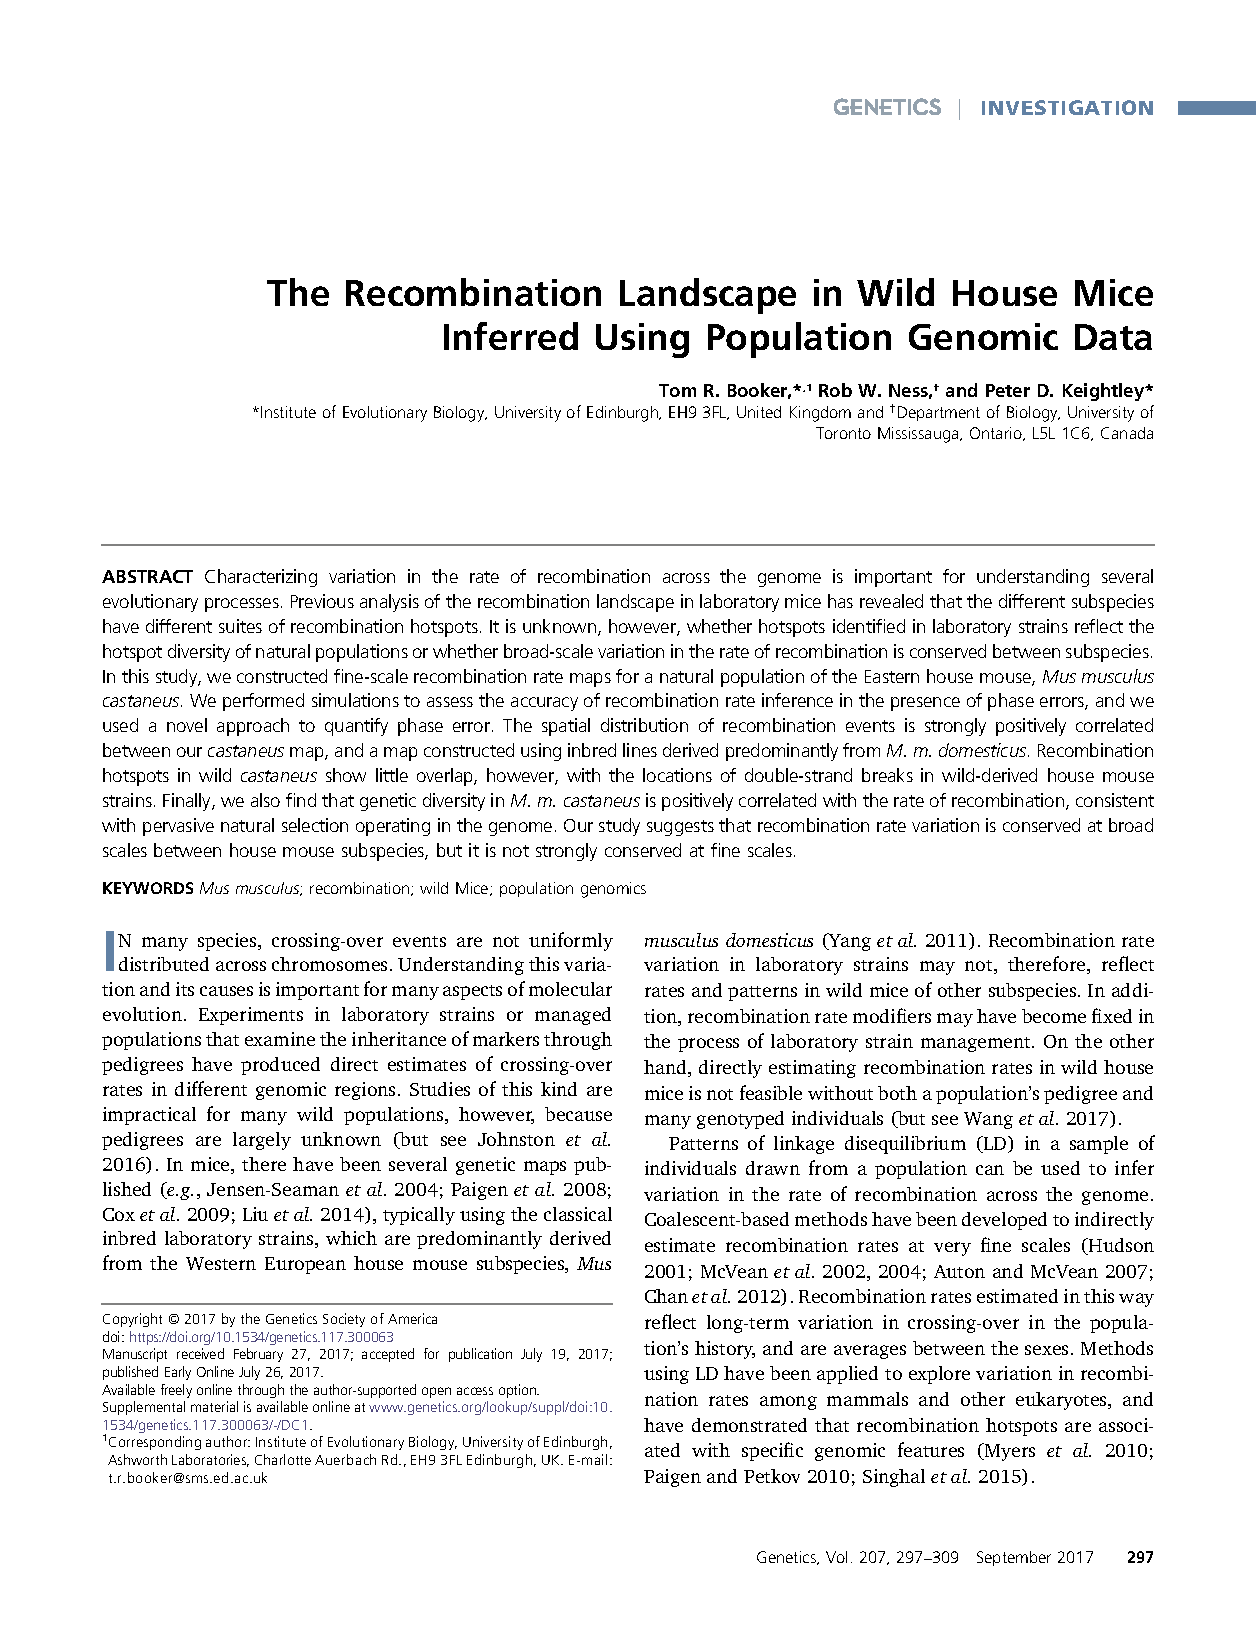
\includepdf[pages=-, scale = 0.8 , pagecommand={\pagestyle{fancy}}]{/Users/s0784966/Dropbox/Thesis/chapter2Appendix/Booker_et_al2017_Genetics.pdf}